%%%%%%%%%%%%%%%%%%%%%%%%%%%%%% Preamble
\documentclass[11pt]{article}
\setlength{\parskip}{\baselineskip}%
\setlength{\parindent}{0pt}%
\usepackage{amsmath,amssymb,amsthm,physics,graphicx,titling}
\usepackage{fontspec}
\setmainfont{Humor Sans}
\newcommand{\subtitle}[1]{%
  \posttitle{%
    \par\end{center}
    \begin{center}\large#1\end{center}
    \vskip0.5em}%
}

\usepackage{graphicx}
\begin{document}

%%%%%%%%%%%%%%%%%%%%%%%%%%%%%% Heading
	\title{Ph 20 - Assignment 1}
	\author{Yovan Badal}
	\date{10/09/2017}
	\maketitle
	
%%%%%%%%%%%%%%%%%%%%%%%%%%%%%% Body
\section{Lissajous Figures}
We observe some Lissajous curves that demonstrate that the figures are closed curves if $\frac{f_X}{f_Y}$ is a rational number for the parametric functions $X(t)   =A_X \cos(2\pi f_X t)$ and $Y(t)   =A_Y \sin(2\pi f_Y t + \phi)$ plotted against each other.

\begin{figure}[htp]
\centering
	\begin{minipage}{0.45\textwidth}
	\centering
	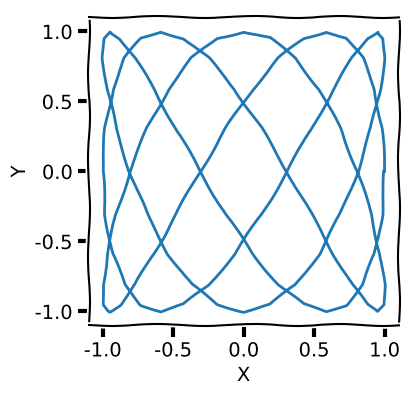
\includegraphics[width=0.9\textwidth]{lissajous_3_5_1_1_0_0.01_100.png}
	\caption{Plot of Y against X for $\frac{f_X}{f_Y}=\frac{3}{5}$.}
	\label{ratio35}
	\end{minipage}\hfill	
	\begin{minipage}{0.45\textwidth}
	\centering
	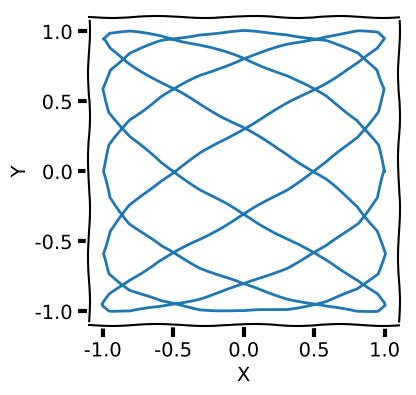
\includegraphics[width=0.9\textwidth]{lissajous_5_3_1_1_0_0.01_100.png}
	\caption{Plot of Y against X for $\frac{f_X}{f_Y}=\frac{5}{3}$.}
	\label{ratio53}
	\end{minipage}
\end{figure}
\newpage

\begin{figure}[htp]
\centering
	\begin{minipage}{0.45\textwidth}
	\centering
	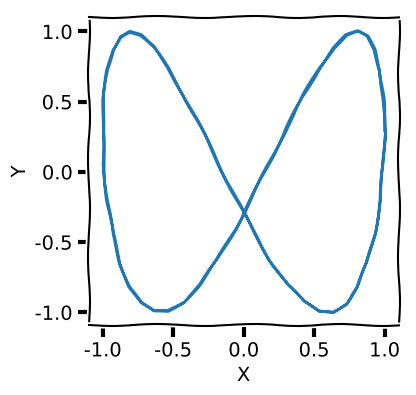
\includegraphics[width=0.9\textwidth]{lissajous_2_4_1_1_0.3_0.01_100.png}
	\caption{Plot of Y against X for $\frac{f_X}{f_Y}=\frac{1}{2}$.}
	\label{ratio0.5}
	\end{minipage}\hfill	
	\begin{minipage}{0.45\textwidth}
	\centering
	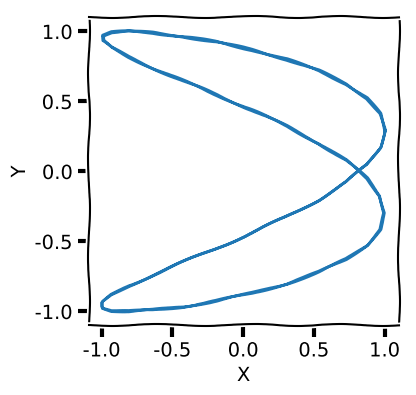
\includegraphics[width=0.9\textwidth]{lissajous_4_2_1_1_0.3_0.01_100.png}
	\caption{Plot of Y against X for $\frac{f_X}{f_Y}=2$.}
	\label{ratio5}
	\end{minipage}
\end{figure}

We observe that for the above plots where $\frac{f_X}{f_Y}$ is a rational number, the Lissajous curves are closed. 

Note: Fig. 3 and 4 have been generated with $\phi=0.3$. This is simply to make it clear that these curves are closed. If we consider the case where $\phi=0$, we can have curves like these:
\begin{figure}[htp]
\centering
	\begin{minipage}{0.45\textwidth}
	\centering
	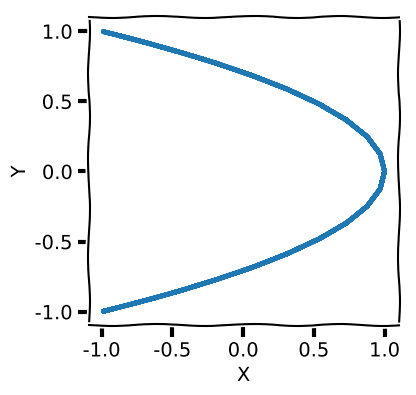
\includegraphics[width=0.9\textwidth]{lissajous_4_2_1_1_0_0.01_1000.png}
	\caption{Plot of Y against X for $\frac{f_X}{f_Y}=2$ and $N=1000$.}
	\label{ratio2_nophi_1000}
	\end{minipage}\hfill	
	\begin{minipage}{0.45\textwidth}
	\centering
	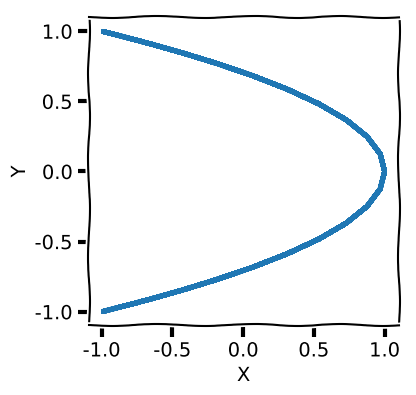
\includegraphics[width=0.9\textwidth]{lissajous_4_2_1_1_0_0.01_10000.png}
	\caption{Plot of Y against X for $\frac{f_X}{f_Y}=2$ and $N=10000$.}
	\label{ratio2_nophi_10000}
	\end{minipage}
\end{figure}

This type of curve may appear open at first, but is in fact closed (the return path is the same as the initial path). We can easily confirm this by plotting over larger $N$, and observing that the curve appears dense (therefore, not closed) for irrational $\frac{f_X}{f_Y}$ but not for rational $\frac{f_X}{f_Y}$.

\begin{figure}[htp]
\centering
	\begin{minipage}{0.45\textwidth}
	\centering
	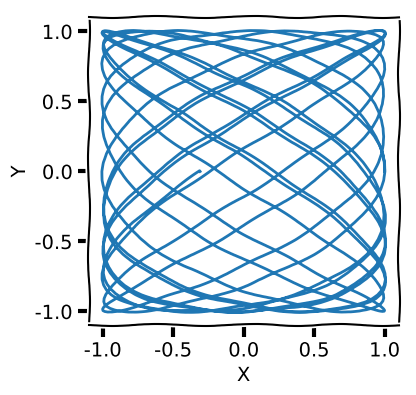
\includegraphics[width=0.9\textwidth]{lissajous_1.57_1_1_1_0_0.01_1000.png}
	\caption{Plot of Y against X for $\frac{f_X}{f_Y}=\pi$ and $N=1000$.}
	\label{ratio1.57}
	\end{minipage}\hfill	
	\begin{minipage}{0.45\textwidth}
	\centering
	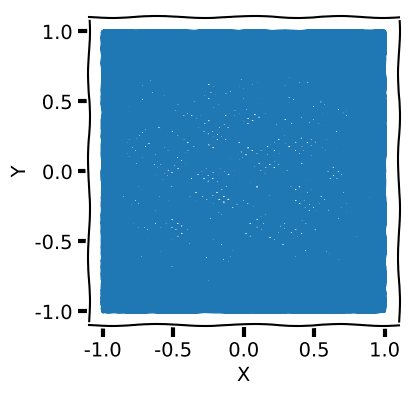
\includegraphics[width=0.9\textwidth]{lissajous_1.57_1_1_1_0_0.01_10000.png}
	\caption{Plot of Y against X for $\frac{f_X}{f_Y}=\pi$ and $N=10000$.}
	\label{ratio1.57_2}
	\end{minipage}
\end{figure}

From figures 1-6, we can get an idea of the relationship between the ratio $\frac{f_X}{f_Y}$ and the shape of the resulting Lissajous curve. We observe that if we express $\frac{f_X}{f_Y}$ as a fraction in its lowest terms, the numerator corresponds to the number of peaks pointing in a direction parallel to the X-axis (the same number of peaks point in a direction antiparallel to the X-axis), and the denominator corresponds to the number of peaks pointing in a direction parallel to the Y-axis (the same number of peaks point in a direction antiparallel to the Y-axis).
\newpage

\section{Beats}
\begin{figure}[htp]
\centering
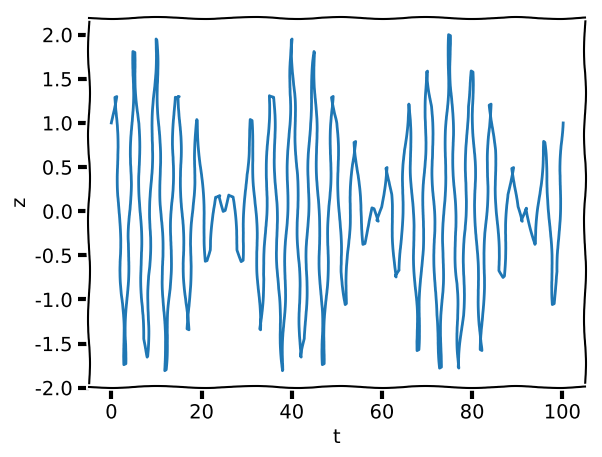
\includegraphics[scale=0.8]{beats_20_23_1_1_0_0.01_100.png}
\caption{Plot of $Z(t)$ with $f_X=20$ and $f_Y=23$, demonstrating the phenomenon of beats.}
\label{beats20_23}
\end{figure}

When $f_X$ and $f_Y$ are nearby, the function $Z(t)$ can be approximated by
\[
Z(t) = 2 \cos (\frac{\omega_1 + \omega_2}{2} t) \cos (\frac{\omega_1 - \omega_2}{2} t).
\]
Although the frequency of the modulating term is $\frac{\omega_1 - \omega_2}{2}$, the modulation does not depend on the value of that term, but rather on its absolute value. This is because having a negative modulation term (as opposed to a positive one) inverts the carrier waveform but maintains its amplitude as compared to that for a positive modulating term.

The modulation cycles therefore have frequency twice that of the modulating term, $\omega_1-\omega_2$.
\newpage

\section{Programming in Python}
I have some (admittedly limited) familiarity with Python from a previous class. I found it very easy to learn the first time, and very easy to re-learn after months of unuse. I definitely agree with Guido van Rossum that Python's approach to object-oriented programming is simple but effective (although the CS people I've talked to since learning Python seem to complain about its computational efficiency, but I know little about that and it doesn't matter much for the purposes I've used it for and am likely to use it for for this class). Its shallow learning-curve and simple, clear syntax make it easy to debug and therefore, in my opinion, a good language to run quick analyses and simulations. It's greatest advantage so far has been Python's modularity. Using the numpy library has made my code for the Lissajous curves much easier to write, debug and handle. I'm sure learning to use more libraries will improve productivity further.

The only other programming language I am familiar with is the Wolfram Language (another computational efficiency pet peeve of said CS people). I enjoy using the Wolfram Language for my coursework and research, mostly because it allows me to do so much with so little writing - often several lines of code in another language (for instance, this week's assignment) can be reduced to 1-2 lines of Wolfram code due to the sheer breadth of built-in functions. This allows me to play around with parameters and visualize models very easily, but comes at the cost of clarity of code, modularity, and ease of debugging. This combination often results in having to test my code line by line, function by function, and argument by argument. Python's clear syntax and allowing for modularity made code refreshingly easy to test and modify.

\end{document}